\documentclass[11pt]{article}

\usepackage[a4paper, lmargin=1cm, rmargin=1cm, tmargin=2cm, bmargin=3cm]{geometry}
\usepackage[utf8]{inputenc}
\usepackage[english]{babel}
\usepackage{graphicx}
\usepackage{amssymb}
\usepackage[hidelinks]{hyperref}
\usepackage{xcolor}
\definecolor{dark-blue}{rgb}{0.15,0.15,0.4}
\hypersetup{colorlinks, linkcolor={dark-blue}, citecolor={dark-blue}, urlcolor={dark-blue}}
\usepackage{changepage}  % \begin{adjustwidth}
\usepackage{multicol}  % \begin{multicols}{2}

\setlength{\parindent}{0cm}
\setlength{\parskip}{1em}

\usepackage{lastpage}
\usepackage{fancyhdr}
\pagestyle{fancy}
\renewcommand{\headrulewidth}{0pt}
\fancyfoot[L]{Last update: \today}
\fancyfoot[C]{}
\fancyfoot[R]{Page \thepage\ of \pageref{LastPage}}

\usepackage{tikz}
\usetikzlibrary{tikzmark, calc}



\begin{document}

%%%%%%%%%%%%%%%%%%%%%%% PERSONAL INFO %%%%%%%%%%%%%%%%%%%%%%%%%

\begin{tikzpicture}[remember picture,overlay]
\fill[blue!10] (current page.north west) rectangle ([yshift=-37ex]current page.north east);
\end{tikzpicture}

\vspace{-12ex}
\makebox[\textwidth]{%
\begin{minipage}[t]{0.3\textwidth}
\centering
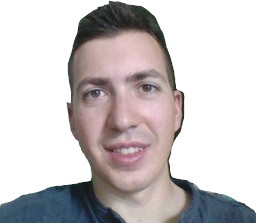
\includegraphics[width=10em]{imgs/photo}

\bigskip
\begin{minipage}{13em}
$\bullet$ Machine learning specialist\\
$\bullet$ Computer vision specialist\\
$\bullet$ Programmer
\end{minipage}
\end{minipage}\hfill%
\begin{minipage}[t]{0.6\textwidth}
\vspace{-12ex}
\textbf{\Huge Ricardo Cruz}\\[6.5ex]
\raisebox{-0.25\height}{
\includegraphics{imgs/icon-geo}} Valongo, Portugal\\
\raisebox{-0.25\height}{
\includegraphics{imgs/icon-phone}} +351 934741617\\
\raisebox{-0.25\height}{
\includegraphics{imgs/icon-mail}} \href{mailto:ricardo.pdm.cruz@gmail.com}{\tt ricardo.pdm.cruz@gmail.com}\\
\raisebox{-0.25\height}{
\includegraphics{imgs/icon-home}} \url{http://rpmcruz.github.io}
\end{minipage}}

%%%%%%%%%%%%%%%%%%%%%%% SUMMARY %%%%%%%%%%%%%%%%%%%%%%%%%

\vspace{2ex}

For the last few years, I have been working at INESC TEC -- an institute that does both academic research and industry development. I have been doing both machine learning and computer vision, working in TensorFlow, PyTorch, and OpenCV.

I have just completed my Ph.D. in Computer Science (june 2021). During the Ph.D., I have been serving a few hours per week as a Teacher Assistant at the Faculty of Engineering, University of Porto, helping teach Python and C++. In 2021, I was awarded the Pedagogy Award based on student feedback.

\centerline{\rule{0.4\linewidth}{0.2pt}}

%%%%%%%%%%%%%%%%%%%%%%% SKILLS %%%%%%%%%%%%%%%%%%%%%%%%%

\begin{minipage}[t]{0.08\linewidth}
\textsc{Skills:}
\end{minipage}
\begin{minipage}[t]{0.92\linewidth}
\small
Python $\cdot$ C $\cdot$ C++ $\cdot$ Java $\cdot$ R $\cdot$ MATLAB $\cdot$ TensorFlow $\cdot$ PyTorch $\cdot$ OpenCV $\cdot$ SQL $\cdot$ Git
\end{minipage}

%%%%%%%%%%%%%%%%%%%%%%% WORK (part 1) %%%%%%%%%%%%%%%%%%%%%%%%%

\begin{minipage}[t]{0.55\textwidth}
\setlength{\parskip}{1em}
\centerline{\sc\large Work Experience}

\begin{samepage}\tikzmark{work1}\textbf{Oct. 2015--Jul. 2021} $\vert$ INESC TEC
\\\tikzmark{work1}{\small Machine Learning Specialist}\begin{adjustwidth}{1.5em}{}%
\footnotesize
INESC TEC is an R\&D institute whose headquarters are located in Porto. I collaborated in the following projects:\par\tikzmark{work11}\textbf{2020--2021 CadPath.AI:} high-performing computing plataform in collaboration with IMP for molecular diagnosis of cancer cells
\tikz[overlay, remember picture] \draw[dashed, black!60] ([shift={(0.5em,-1ex)}]pic cs:work1) |- ([shift={(-0.3em,0.7ex)}]pic cs:work11);\\\tikzmark{work12}\textbf{2018--2020 CLARE:} low-cost mobile device for cervical cancer diagnosis in collaboration with Fraunhofer
\tikz[overlay, remember picture] \draw[dashed, black!60] ([shift={(0.5em,-1ex)}]pic cs:work1) |- ([shift={(-0.3em,0.7ex)}]pic cs:work12);\\\tikzmark{work13}\textbf{2015--2017 NanoSTIMA:} medical machine learning systems, in collaboration with CINTESIS, FMUP and IBMC
\tikz[overlay, remember picture] \draw[dashed, black!60] ([shift={(0.5em,-1ex)}]pic cs:work1) |- ([shift={(-0.3em,0.7ex)}]pic cs:work13);\\\tikzmark{work14}Internal awards
\tikz[overlay, remember picture] \draw[dashed, black!60] ([shift={(0.5em,-1ex)}]pic cs:work1) |- ([shift={(-0.3em,0.7ex)}]pic cs:work14);\begin{adjustwidth}{1.5em}{}%
\footnotesize
\vspace{-2ex}\tikzmark{work141}2021 march: outstanding recognition award
\tikz[overlay, remember picture] \draw[dashed, black!60] ([shift={(0.5em,-1ex)}]pic cs:work14) |- ([shift={(-0.3em,0.7ex)}]pic cs:work141);\\{\footnotesize \url{https://bip.inesctec.pt/en/especiaisdecorrida/ricardo-cruz-ctm-2/}}\\\tikzmark{work142}2018 sept: outstanding recognition award
\tikz[overlay, remember picture] \draw[dashed, black!60] ([shift={(0.5em,-1ex)}]pic cs:work14) |- ([shift={(-0.3em,0.7ex)}]pic cs:work142);\\{\footnotesize \url{http://bip-archive.inesctec.pt/en/196/fora-de-serie.html}}\\
\end{adjustwidth}

\end{adjustwidth}
\end{samepage}\begin{samepage}\tikzmark{work2}\textbf{Sept. 2018--Aug. 2021} $\vert$ FEUP
\\\tikzmark{work2}{\small Teacher Assistant (part-time)}\begin{adjustwidth}{1.5em}{}%
\footnotesize
\tikzmark{work21}Teaching Python (EIC0005) and C/C++ (EIC0012) for MIEIC
\tikz[overlay, remember picture] \draw[dashed, black!60] ([shift={(0.5em,-1ex)}]pic cs:work2) |- ([shift={(-0.3em,0.7ex)}]pic cs:work21);\\\tikzmark{work22}2021: received FEUP pedagogic award, voted by students
\tikz[overlay, remember picture] \draw[dashed, black!60] ([shift={(0.5em,-1ex)}]pic cs:work2) |- ([shift={(-0.3em,0.7ex)}]pic cs:work22);\\
\end{adjustwidth}
\end{samepage}\begin{samepage}\tikzmark{work3}\textbf{Mar.--Jul. 2015} $\vert$ Flykt Startup
\begin{adjustwidth}{1.5em}{}%
\footnotesize
I was involved in a non-successful startup whose goal was to search for travel destinations. I was involved in the NLP part.\par\end{adjustwidth}
\end{samepage}
\end{minipage}
%
\hfill\raisebox{-0.54\textheight}{\rule{0.5pt}{0.55\textheight}}\hfill%
%%%%%%%%%%%%%%%%%%%%%%% EDUCATION %%%%%%%%%%%%%%%%%%%%%%%%%
%
\begin{minipage}[t]{0.40\textwidth}
\setlength{\parskip}{1em}
\centerline{\sc\large Education}

\begin{samepage}\tikzmark{education1}\textbf{2016--2021} $\vert$ Ph.D. in Computer Science
\\\tikzmark{education1}{\footnotesize University of Porto, Minho and Aveiro (joint degree)}\begin{adjustwidth}{1.5em}{}%
\footnotesize
\tikzmark{education11}Thesis title: Re-thinking a Deep Learning Pipeline for Images
\tikz[overlay, remember picture] \draw[dashed, black!60] ([shift={(0.5em,-1ex)}]pic cs:education1) |- ([shift={(-0.3em,0.7ex)}]pic cs:education11);\\\tikzmark{education12}Supervisors: Jaime S. Cardoso and Joaquim F. Pinto Costa
\tikz[overlay, remember picture] \draw[dashed, black!60] ([shift={(0.5em,-1ex)}]pic cs:education1) |- ([shift={(-0.3em,0.7ex)}]pic cs:education12);\\\tikzmark{education13}12 publications, 1 best paper award
\tikz[overlay, remember picture] \draw[dashed, black!60] ([shift={(0.5em,-1ex)}]pic cs:education1) |- ([shift={(-0.3em,0.7ex)}]pic cs:education13);\\
\end{adjustwidth}
\end{samepage}\begin{samepage}\tikzmark{education2}\textbf{2013--2015} $\vert$ MSc in Mathematical Engineering
\\\tikzmark{education2}{\footnotesize Faculty of Sciences, University of Porto}\begin{adjustwidth}{1.5em}{}%
\footnotesize
\tikzmark{education21}Graduated with honors: 18 out of 20 points
\tikz[overlay, remember picture] \draw[dashed, black!60] ([shift={(0.5em,-1ex)}]pic cs:education2) |- ([shift={(-0.3em,0.7ex)}]pic cs:education21);\\
\end{adjustwidth}
\end{samepage}\begin{samepage}\tikzmark{education3}\textbf{2009--2012} $\vert$ BSc in Computer Science
\\\tikzmark{education3}{\footnotesize Faculty of Sciences, University of Porto}\begin{adjustwidth}{1.5em}{}%
\footnotesize
\tikzmark{education31}Graduated with honors: 16 out of 20 points
\tikz[overlay, remember picture] \draw[dashed, black!60] ([shift={(0.5em,-1ex)}]pic cs:education3) |- ([shift={(-0.3em,0.7ex)}]pic cs:education31);\\
\end{adjustwidth}
\end{samepage}
\end{minipage}

%%%%%%%%%%%%%%%%%%%%%%% WORK (cont'd) %%%%%%%%%%%%%%%%%%%%%%%%%

\newpage
\centerline{\sc\large Work Experience (cont'd)}
\begin{multicols}{2}
\setlength{\columnseprule}{0.4pt}
\begin{samepage}\tikzmark{workc1}\textbf{Sept. 2014--Feb. 2015} $\vert$ Research Grant
\\\tikzmark{workc1}{\small Mathematics Center of the University of Porto}\begin{adjustwidth}{1.5em}{}%
\footnotesize
Research on epidemiological models: from differential equations to stochastic simulations and cellular automata.\par\end{adjustwidth}
\end{samepage}
\end{multicols}

%%%%%%%%%%%%%%%%%%%%%%% WORKSHOPS %%%%%%%%%%%%%%%%%%%%%%%%%

\bigskip
\centerline{\sc\large Some of my Workshops}
\begin{multicols}{2}
\setlength{\columnseprule}{0.4pt}
\begin{samepage}\tikzmark{workshops1}\textbf{May 2021} $\vert$ IEEE Bioengeering Society (EMBS - ISEL)
\\\tikzmark{workshops1}{\small Scikit-image and scikit-learn}\par\end{samepage}\begin{samepage}\tikzmark{workshops2}\textbf{Oct 2019} $\vert$ DSPT Day
\\\tikzmark{workshops2}{\small Lightning talk on class imbalance}\par\end{samepage}\begin{samepage}\tikzmark{workshops3}\textbf{August 2018} $\vert$ Universidade Junior
\\\tikzmark{workshops3}{\small "Escondidos nos Dados:'' Teaching data science to highschool students}\par\end{samepage}\begin{samepage}\tikzmark{workshops4}\textbf{August 2018} $\vert$ Porto Codes Meetups
\\\tikzmark{workshops4}{\small Building a Neural Network}\par\end{samepage}\begin{samepage}\tikzmark{workshops5}\textbf{Sept 2017} $\vert$ Porto Codes Meetups
\\\tikzmark{workshops5}{\small Julia Programming Language}\par\end{samepage}\begin{samepage}\tikzmark{workshops6}\textbf{June 2017} $\vert$ Python Meetup
\\\tikzmark{workshops6}{\small NumPy and Scikit-Learn}\par\end{samepage}\begin{samepage}\tikzmark{workshops7}\textbf{Oct 2016} $\vert$ FEUP Code Week
\\\tikzmark{workshops7}{\small Python for scientific computing}\par\end{samepage}
\end{multicols}

%%%%%%%%%%%%%%%%%%%%%%% OPEN-SOURCE %%%%%%%%%%%%%%%%%%%%%%%%%

\bigskip
\centerline{\sc\large Selected Open-Source Portfolio}
\begin{multicols}{2}
\setlength{\columnseprule}{0.4pt}
\begin{samepage}\tikzmark{opensource1}\textbf{2017} $\vert$ Avito NLP competition @ Kaggle
\\\tikzmark{opensource1}{\small Bronze award for results and silver award for engagement}\par\end{samepage}\begin{samepage}\tikzmark{opensource2}\textbf{2010} $\vert$ Apoo, a virtual machine
\\{\footnotesize\begin{minipage}{0.35\linewidth}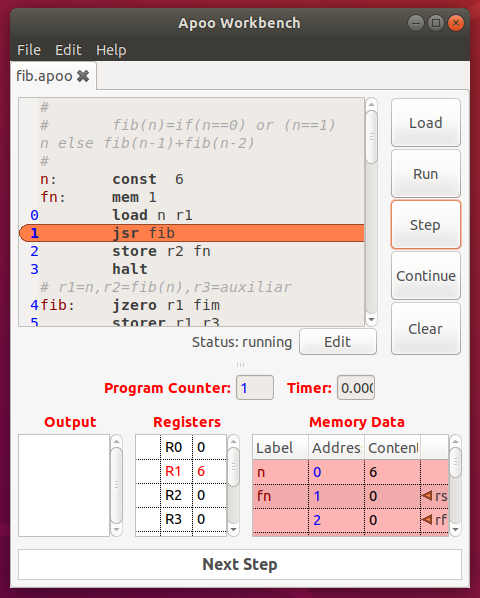
\includegraphics[width=\linewidth]{imgs/cv-apoo.png}\end{minipage}\hfill\begin{minipage}{0.64\linewidth}I helped with the development of Apoo (together with Profs Rogério Reis and Nelma Moreira), a virtual machine that is currently being used to teach Assembly. Apoo is written in Python and GTK+.\end{minipage}}\par\end{samepage}\begin{samepage}\tikzmark{opensource3}\textbf{2009} $\vert$ EatFeed
\\\tikzmark{opensource3}{\small RSS/Atom reader written in C++ and GTK+}\\{\footnotesize \url{https://github.com/rpmcruz/eatfeed}}\\{\footnotesize\begin{minipage}{0.35\linewidth}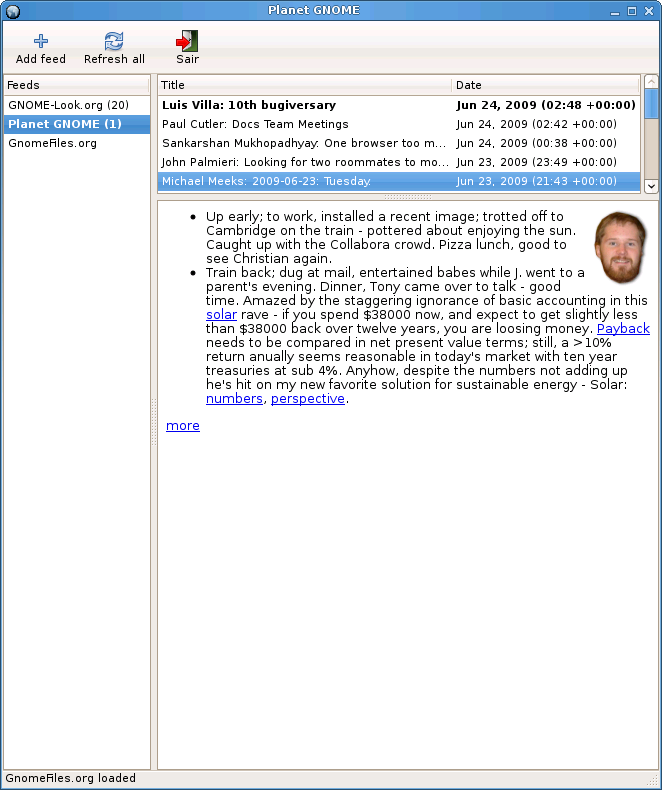
\includegraphics[width=\linewidth]{imgs/cv-eatfeed.png}\end{minipage}}\par\end{samepage}\begin{samepage}\tikzmark{opensource4}\textbf{2006 and 2007} $\vert$ Google Summer of Code
\begin{adjustwidth}{1.5em}{}%
\footnotesize
\tikzmark{opensource41}2007: LibreOffice dynamic layouts (C++)
\tikz[overlay, remember picture] \draw[dashed, black!60] ([shift={(0.5em,-1ex)}]pic cs:opensource4) |- ([shift={(-0.3em,0.7ex)}]pic cs:opensource41);\\\tikzmark{opensource42}2006: YaST port from GTK+ to Qt (C++)
\tikz[overlay, remember picture] \draw[dashed, black!60] ([shift={(0.5em,-1ex)}]pic cs:opensource4) |- ([shift={(-0.3em,0.7ex)}]pic cs:opensource42);\\
\end{adjustwidth}
\end{samepage}\begin{samepage}\tikzmark{opensource5}\textbf{2005} $\vert$ J2ME and Android games
\\{\footnotesize \url{https://github.com/rpmcruz/android-games}}\begin{adjustwidth}{1.5em}{}%
\footnotesize
Games written in Java Mobile Edition; more recently, I ported a couple of them to Android.\par\end{adjustwidth}
\end{samepage}\begin{samepage}\tikzmark{opensource6}\textbf{2005} $\vert$ SuperTux, co-author
\\{\footnotesize \url{https://www.supertux.org/}}\\{\footnotesize\begin{minipage}{0.35\linewidth}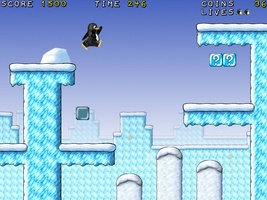
\includegraphics[width=\linewidth]{imgs/cv-supertux.jpg}\end{minipage}\hfill\begin{minipage}{0.64\linewidth}While in high-school, I was part of the initial team developing this game. It is written in C++, SDL, and OpenGL.\end{minipage}}\par\end{samepage}
\begin{itemize}
\small
\renewcommand{\labelitemi}{$\blacktriangleright$}
\setlength{\itemindent}{-1.5em}
\itemsep0em 
\item Find more of my open-source code at\\\href{https://github.com/rpmcruz?tab=repositories}{\tt https://github.com/rpmcruz}.
\item Videos showing some of my work: \url{https://www.youtube.com/channel/UCLS6OCVgk_qPohhUqSPvLJw}.
\end{itemize}
\end{multicols}

%%%%%%%%%%%%%%%%%%%%%%% PUBLICATIONS %%%%%%%%%%%%%%%%%%%%%%%%%

\newpage
\centerline{\sc\large Publications}
These are my indexed publications (some publications in \textbf{bold} for emphasis).
\begin{enumerate}
\itemsep0em
\item 2021. ``Ordinal Losses for Classification of Cervical Cancer Risk.'' T. Albuquerque, R. Cruz, J. Cardoso. PeerJ Computer Science.\item \textbf{2021. ``Background Invariance by Adversarial Learning.'' R. Cruz, R. Prates, E. Filho, J. Costa, J. Cardoso. 25th International Conference on Pattern Recognition (ICPR), IEEE.}\item 2019. ``Automatic Augmentation by Hill Climbing.'' R. Cruz, J. Costa, J. Cardoso. 28th International Conference on Artificial Neural Networks (ICANN), Springer.\item \textbf{2019. ``Averse Deep Semantic Segmentation.'' R. Cruz, J. Costa, J. Cardoso. 41st Engineering in Medicine and Biology Conference (EMBC), IEEE.}\item 2019. ``Insulator visual non-conformity detection in overhead power distribution lines using deep learning.'' R. Prates, R. Cruz, A. Marotta, R. Ramos, E. Filho, J. Cardoso. Journal Computers \& Electrical Engineering, Springer.\item 2018. ``A Class Imbalance Ordinal Method for Alzheimer's Disease Classification.'' R. Cruz, M. Silveira, J. Cardoso. 2018 International Workshop on Pattern Recognition in Neuroimaging (PRNI), IEEE.\item 2018. ``Binary ranking for ordinal class imbalance.'' R. Cruz, K. Fernandes, J. Costa, M. Pérez Ortiz, J. Cardoso. Journal Pattern Analysis and Applications, Springer.\item \textbf{2018. ``Deep image segmentation by quality inference.'' K. Fernandes, R. Cruz, J. Cardoso. International Joint Conference on Neural Networks (IJCNN), IEEE.}\item 2017. ``Constraining type II error: building intentionally biased classifiers.'' R. Cruz, K. Fernandes, J. Costa, J. Cardoso. International Work-conference on Artificial Neural Networks (IWANN), Springer.\item 2017. ``Fine-to-coarse ranking in ordinal and imbalanced domains: an application to liver transplantation.'' M. Pérez-Ortiz, K. Fernandes, R. Cruz, J. Cardoso. International Work-conference on Artificial Neural Networks (IWANN), Springer.\item 2017. ``Combining ranking with traditional methods for ordinal class imbalance.'' R. Cruz, K. Fernandes, J. Costa, M. Pérez-Ortiz, J. Cardoso. International Work-conference on Artificial Neural Networks (IWANN), Springer.\item 2017. ``Ordinal class imbalance with ranking.'' R. Cruz, K. Fernandes, J. Costa, M. Pérez-Ortiz, J. Cardoso. Iberian conference on pattern recognition and image analysis (Ibpria), Springer.\item \textbf{2016. ``Tackling class imbalance with ranking.'' R. Cruz, K. Fernandes, J. Costa, J. Cardoso. International Joint Conference on Neural Networks (IJCNN), IEEE.}\end{enumerate}
My Google Scholar: \url{https://scholar.google.pt/citations?user=pSFY_gQAAAAJ}

\end{document}
